\documentclass[a4paper,12pt]{article}

\usepackage[T2A]{fontenc}
\usepackage[utf8]{inputenc}
\usepackage[english,russian]{babel}
\usepackage{amsmath}
\usepackage{pgfplots}
\usepackage{geometry}
\usepackage{graphicx}
\usepackage[section,above,below]{placeins}
\usepackage{afterpage,placeins}
\usepackage{booktabs}
\usepackage{listings}
\usepackage{color}

\usepackage{algorithm}
\usepackage[noend]{algpseudocode}

\DeclareGraphicsExtensions{.png,.jpg}

\geometry{left=2cm}
\geometry{right=1.5cm}
\geometry{top=1cm}
\geometry{bottom=1.5cm}

\headheight = 1cm
\footskip = 0pt

\parskip = 4.25mm % расстояние между строками
\parindent=6.375mm % расстояние между абзацами
\floatname{algorithm}{Алгоритм} % переопределение имени в псевдокоде

\begin{document}
    \begin{titlepage}
        \begin{center}
            \large
            Государственное образовательное учреждение высшего профессионального образования\\
            “Московский государственный технический университет имени Н.Э.Баумана”
            \vspace{3cm}
            
            \textsc{Дисциплина: Анализ алгоритмов}
            \vspace{0.5cm}
                
            \textsc{Лабораторная работа №4}
            \vspace{3cm}
            
            {\LARGE Параллельная реализация алгоритма Винограда}
            \vspace{3cm}
            
            Студент группы ИУ7-54Б,\\   
            Котов Никита
            \vfill
            
            2019 г.            
            \end{center}
    \end{titlepage}
    
    \begin{center}
    	\tableofcontents
    \end{center}
	
	\setcounter{page}{2}
	\newpage
    \begin{center}
        \section*{Введение}
        \addcontentsline{toc}{section}{Введение}
    \end{center}
        \label{sec:intro}
\quad Многопоточность - способность центрального процессора (CPU) или одного ядра в многоядерном процессоре одновременно выполнять несколько процессов или потоков, соответствующим образом поддерживаемых операционной системой. Этот подход отличается от многопроцессорности, так как многопоточность процессов и потоков совместно использует ресурсы одного или нескольких ядер: вычислительных блоков, кэш-памяти ЦПУ или буфера перевода с преобразованием (TLB).


В тех случаях, когда многопроцессорные системы включают в себя несколько полных блоков обработки, многопоточность направлена на максимизацию использования ресурсов одного ядра, используя параллелизм на уровне потоков, а также на уровне инструкций. Поскольку эти два метода являются взаимодополняющими, их иногда объединяют в системах с несколькими многопоточными ЦП и в ЦП с несколькими многопоточными ядрами.
 
		
Многопоточная парадигма стала более популярной с конца 1990-х годов, поскольку усилия по дальнейшему использованию параллелизма на уровне инструкций застопорились. Смысл многопоточности - квазимногозадачность на уровне одного исполняемого процесса. Значит, все потоки процесса помимо общего адресного пространства имеют и общие дескрипторы файлов. Выполняющийся процесс имеет как минимум один (главный) поток.

Многопоточность (как доктрину программирования) не следует путать ни с многозадачностью, ни с многопроцессорностью, несмотря на то, что операционные системы, реализующие многозадачность, как правило, реализуют и многопоточность.
Достоинства:
\begin{itemize}
    \item облегчение программы посредством использования общего адресного пространства.
    \item меньшие затраты на создание потока в сравнении с процессами.
    \item повышение производительности процесса за счёт распараллеливания процессорных вычислений.
    \item если поток часто теряет кэш, другие потоки могут продолжать использовать неиспользованные вычислительные ресурсы.
\end{itemize}
Недостатки:
\begin{itemize}
    \item несколько потоков могут вмешиваться друг в друга при совместном использовании аппаратных ресурсов
    \item с программной точки зрения аппаратная поддержка многопоточности более трудоемка для программного обеспечения
    \item проблема планирования потоков
    \item специфика использования. Вручную настроенные программы на ассемблере, использующие расширения MMX или AltiVec и выполняющие предварительные выборки данных, не страдают от потерь кэша или неиспользуемых вычислительных ресурсов. Таким образом, такие программы не выигрывают от аппаратной многопоточности и действительно могут видеть ухудшенную производительность из-за конкуренции за общие ресурсы\cite{litlink1}.
\end{itemize}
Несмотря на существующие недостатки, многопоточная парадигма имеет огромный потенциал, поэтому данная лабораторная работа будет посвящена распараллеливанию реализованного ранее алгоритма Винограда для умножения матриц.\\ 		
В рамках выполнения работы необходимо решить следующие задачи:   
		\begin{itemize}
			\item изучить понятие параллельный вычислений;
			\item реализовать последовательный и параллельный алгоритм Винограда;
			\item сравнить временные характеристики реализованных алгоритмов экспериментально; 		
			\item на основании проделанной работы сделать выводы.
		\end{itemize}
    \newpage

    \begin{center}
        \section{Аналитическая часть}
	    \subsection{Описание алгоритма}
    \end{center}
\subsubsection{Алгоритм Винограда}
Рассматривая результат умножения двух матриц очевидно, что каждый элемент в нем представляет собой скалярное произведение соответствующих строки и столбца исходных матриц. Такое умножение допускает предварительную обработку, позволяющую часть работы выполнить заранее.

Рассмотрим два вектора V = (v1, v2, v3, v4) и W = (w1, w2, w3, w4). Их скалярное произведение равно: \begin{equation}V * W = v1w1 + v2w2 + v3w3 + v4w4
\end{equation}

Это равенство можно переписать в виде: \begin{equation}V * W = (v1 + w2)(v2 + w1) + (v3 + w4)(v4 + w3) - v1v2 - v3v4 - w1w2 - w3w4
\end{equation}

Несмотря на то, что второе выражение требует вычисления большего количества операций, чем стандартный алгоритм: вместо четырех умножений - шесть, а вместо трех сложений - десять, выражение в правой части последнего равенства допускает предварительную обработку: его части можно вычислить заранее и запомнить для каждой строки первой матрицы и для каждого столбца второй, то для каждого элемента будет необходимо выполнить лишь первые два умножения и последующие пять сложений, а также дополнительно два сложения. Из-за того, что операция сложения быстрее операции умножения, алгоритм должен работать быстрее стандартного.

    \newpage

    \begin{center}
        \section{Конструкторская часть}
        \subsection{Разработка алгоритмов}
    \end{center}
    \subsubsection{Алгоритм Винограда}
    
    На рис.~\ref{ris:vin1} и рис.~\ref{ris:vin2} приведена схема алгоритма Винограда
	 		\begin{figure}[H]
	 			\centering
	 			{
	 				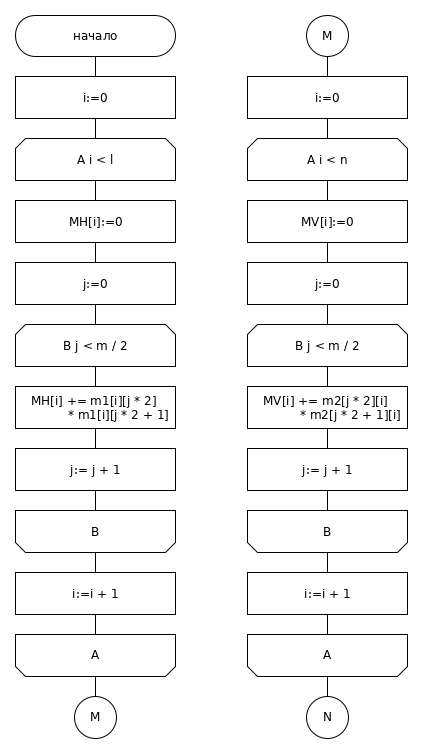
\includegraphics[scale=0.71]{vinograd1.png}
	 				\caption{\label{ris:vin1}Алгоритм Винограда}	
	 			}
	 		\end{figure}	
	 		\begin{figure}[H]
	 			\centering
	 			{
	 				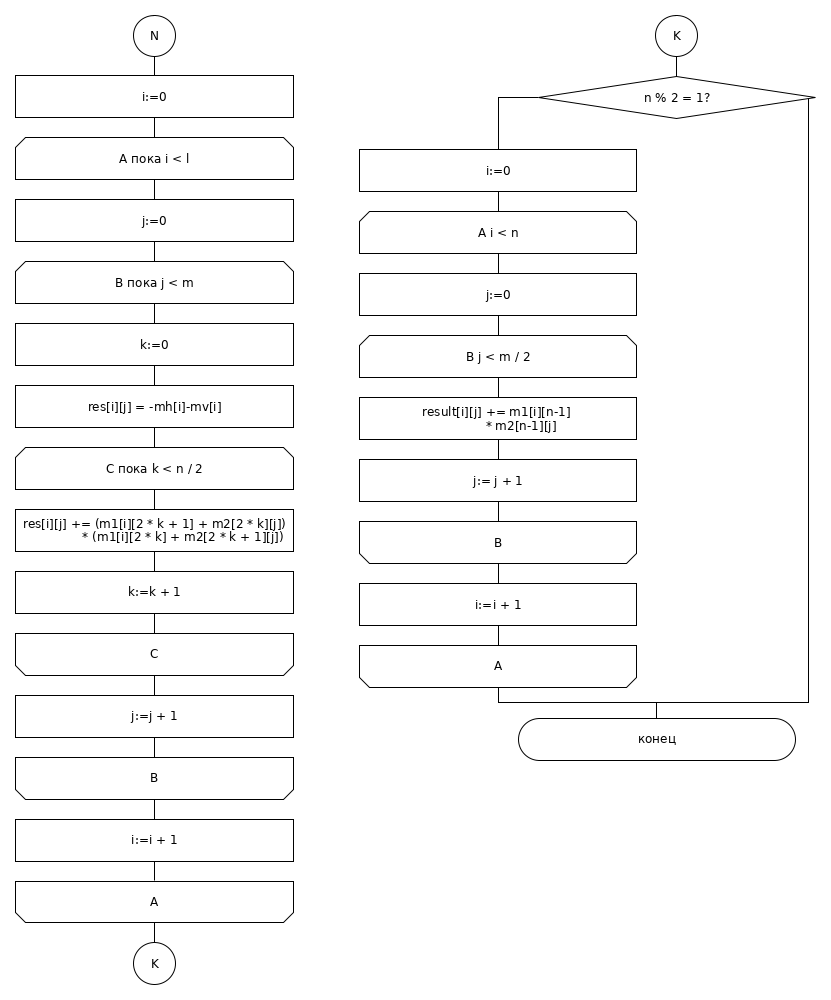
\includegraphics[scale=0.61]{vinograd2.png}
	 				\caption{\label{ris:vin2}Алгоритм Винограда}	
	 			}
	 		\end{figure}
	
	Видно, что для алгоритма Виноградова худшим случаем являются матрицы нечетного размера, а лучшим четного, т.к. отпадает необходимость в последнем цикле.\\
	В качестве оптимизаций можно:
	\begin{itemize}
	\item заранее считать в MH и MV отрицательные произведения
	\item заменить выражения вида $a = a + ...$ на $a += ...$
	\item в циклах по k сделать шаг 2, избавившись тем самым от двух операций умножения на каждую итерацию
	\end{itemize}
	
	Рассмотрим способы распараллеливания алгоритма. 
	\begin{itemize}
		\item Прежде всего предварительные вычисления MH и MV не зависят друг от друга, значит, их можно вычислить параллельно;
		\item Если количество потоков больше 2ух, то вычисления и MH, и MV можно распараллеть, выделив каждому из $n\_threads/2$ потоков, где n\_threads - кол-во доступных потоков, вычисление своего участка длинной $l/n\_threads$ и $n/n\_threads$ соответственно;
		\item Аналогичным способом распараллеливается вычисление матрицы.
	\end{itemize} 
    
    \begin{center}
    	\subsection{Выводы по конструкторскому разделу}    
    \end{center}
   
    	\quad В результате работы над конструкторским разделом была разработана схема алгоритма Винограда и выбран способ распараллеливания алгоритма.
    	
    \newpage
    
    \begin{center}
     	\section{Технологическая часть}
        \subsection{Средства реализации}    
    \end{center}
    
		В качестве языка программирования был выбран C++, так как он предоставляет широкие возможности для эффективной реализации алгоритмов. Для распараллеливания алгоритма выбраны std::thread, предоставляемые стандартно библиотекой С++. Они имеют достаточно удобный интерфейс для поставленных в данной работе задач.
	\begin{center}
	\end{center}

    \begin{center}
        \subsection{Листинг кода}    
    \end{center}
				\lstset{
	        		language=C++,
	        		basicstyle=\ttfamily,
	        		keywordstyle=\color{blue}\ttfamily,
	        		stringstyle=\color{red}\ttfamily,
	        		commentstyle=\color{green}\ttfamily,
	        		morecomment=[l][\color{magenta}]{\#},
	        		columns=fullflexible,
	        	    tabsize=1, 
	        		breakatwhitespace=true
	        	}
        	
\begin{lstlisting}[frame=single,caption=последовательный Алгоритм Винограда, breaklines]
row_d get_negative_row_products(matrix_d &matrix, size_t m, size_t n) {
    auto result = row_d(m, 0.);
    for (size_t i = 0; i < m; i++) {
        for (size_t j = 0; j < n - 1; j += 2) {
            result[i] -= matrix[i][j] * matrix[i][j + 1];
        }
    }

    return result;
}

row_d get_negative_col_products(matrix_d &matrix, size_t m, size_t n) {
    auto result = row_d(m, 0.);
    for (size_t i = 0; i < m; i++) {
        for (size_t j = 0; j < n - 1; j += 2) {
            result[i] -= matrix[j][i] * matrix[j + 1][i];
        }
    }

    return result;
}

matrix_d vinograd_multiplication(matrix_d &m1, matrix_d &m2) {
    auto l = m1.size();
    auto m = m2.size();
    auto n = m2[0].size();

    if (m1[0].size() != m) {
        throw std::exception();
    }

    auto mh = get_negative_row_products(m1, l, m);
    auto mv = get_negative_col_products(m2, n, m);

    auto result = init_matrix(l, n);
    for (size_t i = 0; i < l; i++) {
        for (size_t j = 0; j < m; j++) {
            result[i][j] = mh[i] + mv[j];
            for (size_t k = 0; k < n - 1; k += 2) {
                result[i][j] += (m1[i][k + 1] + m2[k][j]) * (m1[i][k] + m2[k + 1][j]);
            }
        }
    }

    if (n % 2 == 1) {
        for (size_t i = 0; i < l; i++) {
            for (size_t j = 0; j < m; j++) {
                result[i][j] += m1[i][n - 1] * m2[n-1][j];
            }
        }
    }

    return result;
}
\end{lstlisting}
\begin{lstlisting}[frame=single,caption=параллельный Алгоритм Винограда, breaklines]
row_d parallel_negative_row_products(matrix_d &matrix, size_t m, size_t n, size_t threads_num) {
    auto result = row_d(m, 0.);
    auto lambda = [&](size_t i_start, size_t i_end) {
        for (size_t i = i_start; i < i_end; i++) {
            for (size_t j = 0; j < n - 1; j += 2) {
                result[i] -= matrix[i][j] * matrix[i][j + 1];
            }
        }
    };

    std::vector<std::thread> threads(threads_num);
    auto line_for_thread = m / threads_num;
    if (line_for_thread == 0) {
        line_for_thread = 1;
    }

    for (size_t i = 0; i < threads_num && i < m; i++) {
        size_t start = i * line_for_thread;
        size_t end = i == threads_num - 1? m: (i + 1) * line_for_thread;
        auto thread = std::thread(lambda, start, end);
        threads[i] = std::move(thread);
    }

    for (auto &thr: threads) {
        thr.join();
    }

    return result;
}

row_d parallel_negative_col_products(matrix_d &matrix, size_t m, size_t n, size_t threads_num) {
    auto result = row_d(m, 0.);
    auto lambda = [&](size_t i_start, size_t i_end) {
        for (size_t i = i_start; i < i_end; i++) {
            for (size_t j = 0; j < n - 1; j += 2) {
                result[i] -= matrix[j][i] * matrix[j + 1][i];
            }
        }
    };

    std::vector<std::thread> threads(threads_num);
    auto line_for_thread = m / threads_num;
    if (line_for_thread == 0) {
        line_for_thread = 1;
    }

    for (size_t i = 0; i < threads_num && i < m; i++) {
        size_t start = i * line_for_thread;
        size_t end = i == threads_num - 1? m: (i + 1) * line_for_thread;
        auto thread = std::thread(lambda, start, end);
        threads[i] = std::move(thread);
    }

    for (auto &thr: threads) {
        if (thr.joinable()) {
            thr.join();
        }
    }

    return result;
}

matrix_d parallel_vinograd_mult(matrix_d &m1, matrix_d &m2, size_t threads_num) {
    auto l = m1.size();
    auto m = m2.size();
    auto n = m2[0].size();

    if (m1[0].size() != m) {
        throw std::exception();
    }

    row_d mh, mv;
    if (threads_num > 2) {
        std::thread mh_thread([&](){ mh = get_negative_row_products(m1, l, m); });
        std::thread mv_thread([&](){ mv = get_negative_col_products(m2, n, m); });
        mh_thread.join();
        mv_thread.join();
    } else {
        mh = parallel_negative_row_products(m1, l, m, threads_num / 2);
        mv = parallel_negative_col_products(m2, n, m, threads_num - threads_num / 2);
    }

    std::vector<std::thread> threads(threads_num);
    auto line_for_thread = l / threads_num;
    if (line_for_thread == 0) {
        line_for_thread = 1;
    }

    auto result = init_matrix(l, n);
    for (size_t i = 0; i < threads_num && i < l; i++) {
        size_t start = i * line_for_thread;
        size_t end = i == threads_num - 1? l: (i + 1) * line_for_thread;
        auto thread = std::thread(
            [&](size_t i_start, size_t i_end) {
                for (size_t local_i = i_start; local_i < i_end; local_i++) {
                    for (size_t j = 0; j < m; j++) {
                        result[local_i][j] = mh[local_i] + mv[j];
                        for (size_t k = 0; k < n-1; k += 2) {
                            result[local_i][j] += (m1[local_i][k + 1] + m2[k][j]) * (m1[local_i][k] + m2[k + 1][j]);
                        }
                    }
                }
            }, start, end);
        threads[i] = std::move(thread);
    }

    for (auto &thr: threads) {
        if (thr.joinable()) {
            thr.join();
        }
    }

    if (n % 2 == 1) {
        for (size_t i = 0; i < l; i++) {
            for (size_t j = 0; j < m; j++) {
                result[i][j] += m1[i][n - 1] * m2[n-1][j];
            }
        }
    }

    return result;
}
\end{lstlisting}
    \newpage

	\begin{center}		
		\subsection{Тестирование фунций}
	\end{center}		
	
	В таблице~\ref{tabular:test_rec} приведены тесты для последовательной и параллельной реализаций алгоритма Винограда.
					\begin{table}[H]        		
       				\caption{\label{tabular:test_rec} Тестирование функций}
       				\begin{center}
        			\begin{tabular}{c@{\hspace{7mm}}c@{\hspace{7mm}}c@{\hspace{7mm}}c@{\hspace{7mm}}c@{\hspace{7mm}}}        				
        				\hline
        				Матрица 1 & Матрица 2 &Ожидаемый результат &Посл. алг. & Парал. алг. \\ \hline
        				\vspace{4mm}
        				$\begin{pmatrix}
							1 & 2 & 3\\
							1 & 2 & 3\\
							1 & 2 & 3
						\end{pmatrix}$ &
        				$\begin{pmatrix}
							1 & 2 & 3\\
							1 & 2 & 3\\
							1 & 2 & 3
						\end{pmatrix}$ &
						$\begin{pmatrix}
							6 & 12 & 18\\
							6 & 12 & 18\\
							6 & 12 & 18
						\end{pmatrix}$ & $\surd$ & $\surd$\\
        				\vspace{2mm}
        				\vspace{2mm}
						$\begin{pmatrix}
							1 & 2\\
							1 & 2
						\end{pmatrix}$ &
        				$\begin{pmatrix}
							1 & 2\\
							1 & 2
						\end{pmatrix}$ &
						$\begin{pmatrix}
							3 & 6\\
							3 & 6
						\end{pmatrix}$ & $\surd$ & $\surd$\\
       				\vspace{2mm}
       				\vspace{2mm}
						$\begin{pmatrix}
							2
						\end{pmatrix}$ &
        				$\begin{pmatrix}
							2
						\end{pmatrix}$ &
						$\begin{pmatrix}
							4
						\end{pmatrix}$ & $\surd$ & $\surd$\\
       				\vspace{2mm}
        			\vspace{2mm}
        				$\begin{pmatrix}
							1 & -2 & 3\\
							1 & 2 & 3\\
							1 & 2 & 3
						\end{pmatrix}$ &
        				$\begin{pmatrix}
							-1 & 2 & 3\\
							1 & 2 & 3\\
							1 & 2 & 3
						\end{pmatrix}$ &
						$\begin{pmatrix}
							0 & 4 & 6\\
							4 & 12 & 18\\
							4 & 12 & 18
						\end{pmatrix}$ & $\surd$ & $\surd$\\
       				\vspace{2mm}
        			\end{tabular}
        			\end{center}
        			\end{table}

	\newpage

    \begin{center}
        \section{Экспериментальная часть}        
	    \subsection{Тестирование времени работы функций}	
	\end{center}
	
	    Для измерения времени использовались функции std::chrono, предоставляемые стандартной библиотекой С++. Чтобы исключить случайные отклонения в измеренном времени, измерялось время работы 10 запусков функции и делилось на 10. Замеры проводятся на процессоре с 2 физическими и 4 логическими ядрами i5 7200u.
	    
	    В таблице~\ref{tabular:test_time} приведены замеры времени работы на квадратных матрицах последовательной и параллельной реализаций алгоритма Винограда, на основе них построены графики рис~\ref{ris:test1}.
	\begin{table}[H]
	\caption{\label{tabular:test_time} Время работы реализаций алгоритмов}
	\begin{center}	    
	\begin{tabular}{|c|c|c|c|c|c|c|c|}        			
        				\hline
        				Размер матрицы & 1 поток & 2 потока & 4 потока & 8 потоков & 16 потоков & 32 потока & 64 потока \\
        				\hline
        				100      &0.0028  &0.0024  &0.0020  &0.0023 & 0.0026 & 0.0036 & 0.0069\\
        				200      &0.0283  &0.0226  &0.0155 & 0.0158 & 0.0163 & 0.0181 & 0.0200\\
        				300      &0.1208  &0.0668  &0.0843 & 0.0601 & 0.0619 & 0.0680 & 0.0692\\
        				400      &0.3061  &0.1551  &0.1690 & 0.1491 & 0.1587 & 0.1469 & 0.1657\\ 
        				500      &0.7427  &0.4486  &0.3058 & 0.3075 & 0.3058 & 0.3118 & 0.3594\\
        				600      &1.7297  &1.0926  &1.0023 & 0.7592 & 0.7123 & 0.6617 & 0.6699\\ 
        				700      &2.8254  &1.6326  &1.2640 & 1.3399 & 1.2311 & 1.2575 & 1.3509\\
        				800      &4.6763  &2.4869  &2.9249 & 2.6242 & 2.5122 & 2.4741 & 2.5021\\
        				900      &7.2538  &3.5246  &5.6764 & 5.3094 & 5.2693 & 5.2410 & 5.2160\\
        			   1000      &10.1448 &4.9473  &8.6905 & 8.7452 & 8.7369 & 8.7173 & 8.7413\\          						
        				\hline
	\end{tabular}
	\end{center}
	\end{table}
	\begin{center}
					\begin{figure}[H]	
        				{
        					\centering
        					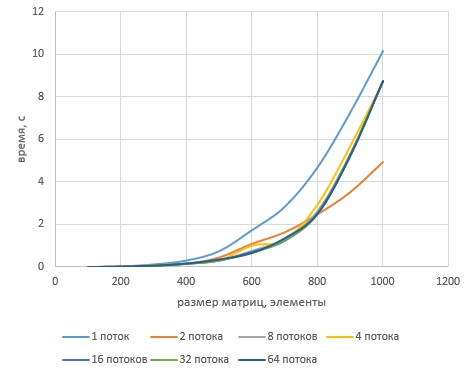
\includegraphics[scale=0.7]{time.jpg}
        					\caption{\label{ris:test1}Замеры времени}
        				}
        			\end{figure}
	\end{center}

	На графике рис.~\ref{ris:test1} видно, что на 2ухпоточный вариант показывает наилучший результат, обгоняя в 2 раза однопоточную реализацию и на 40\% реализации на 4-х и более потоках при размерах матриц от 900х900 и более. Из этого можно сделать вывод, что наиболее эффективно количество потоков равное количеству физических ядер, так как при этом затраты на смену контекстов не снижают производительность.

    \newpage

    \begin{center}
        \section*{Заключение}
        \addcontentsline{toc}{section}{Заключение}
    \end{center}
            \label{sec:ending}
        	\qquad В рамках лабораторной работы было изучено понятие параллельных вычислений. Была реализована параллельная версия алгоритма Винограда и произведены замеры времени ее работы с различным количеством потоков. На основании этого произведено сравнение эффективности параллельной и последовательной версий алгоритма. Наиболее эффективной оказалась параллельная реализация алгоритма Винограда при количестве потоков равном количеству физических ядер процессора, имеющая выйгрыш в 2 раза по скорости по сравнению с последовательной реализации (т.е. в количество физических ядер).
    \newpage

    \begin{center}        
        \begin{thebibliography}{}
        	\bibitem{litlink1}  Введение в технологии параллельного программирования // INTEL: сайт. URL: https://software.intel.com/ru-ru/articles/writing-parallel-programs-a-multi-language-tutorial-introduction/ (дата обращения: 14.10.2019)            	        	
        \end{thebibliography}
    \end{center}

\end{document}
